% !TEX root = ../main.tex
\section{Základní teorémy teorie ODR - Existence, jednoznačnost a kvalitativní vlastnosti}
\label{sec:zakladni-teoremy}

\blocktitle{Cíl kapitoly}
Aplikovat matematický aparát z Kapitoly 2 na fundamentální teorémy existence, jednoznačnosti a kvalitativního chování řešení obyčejných diferenciálních rovnic. Propojit abstraktní funkcionální analýzu s konkrétními dynamickými systémy a kvantovými aplikacemi.

\begin{intermezzo}
\textbf{Navázání na Kapitolu 2:} Zatímco Kapitola 2 poskytla matematický aparát funkcionální analýzy, nyní jej aplikujeme na teorii ODR prostřednictvím \hyperref[sec:matematicky-fundament]{Banachových prostorů pro Picardovu iteraci}, \hyperref[sec:matematicky-fundament]{teorie míry pro Carathéodoryho větu} a \hyperref[sec:matematicky-fundament]{Sobolevových prostorů pro analýzu regularity}.
\end{intermezzo}

\spc

\subsection{Formulace základních problémů a motivace}

\begin{scaffold}
\textbf{Co umíme:} Klasifikace ODR a typy úloh z Kapitoly 1. \\
\textbf{Co se naučíme:} Proč a jak dokazovat existenci a jednoznačnost řešení. \\
\textbf{K čemu to využijeme:} Garance řešení u kvantových a stochastických systémů.
\end{scaffold}

\begin{motivation}
Potřebujeme matematickou jistotu, že naše modely ODR mají smysluplná řešení a že jsou jednoznačná pro dané počáteční podmínky. Bez těchto záruk by jakákoli numerická simulace nebo fyzikální interpretace postrádala pevný základ.
\end{motivation}

\begin{itemize}
\item \textbf{Problém existence:} Existuje alespoň jedno řešení na nějakém intervalu?
\item \textbf{Problém jednoznačnosti:} Je řešení určeno jednoznačně počáteční podmínkou?
\item \textbf{Problém prodloužení:} Lze lokální řešení rozšířit na maximální interval?
\item \textbf{Problém závislosti:} Jak řešení závisí na počátečních podmínkách a parametrech?
\end{itemize}

\begin{intuition}
Geometrický pohled: V fázovém prostoru hledáme křivky (trajektorie), které procházejí daným bodem (počáteční podmínka) a jejichž tečný vektor je dán pravou stranou rovnice. Existence znamená, že z každého bodu vychází alespoň jedna taková křivka, jednoznačnost že právě jedna.
\end{intuition}

\begin{example}[Kvantová motivace]
Pro časově závislou Schrödingerovu rovnici $i\hbar\frac{\partial\psi}{\partial t} = \hat{H}\psi$ potřebujeme garantovat, že pro danou počáteční vlnovou funkci $\psi(0)$ existuje jednoznačné řešení $\psi(t)$ zachovávající normu.
\end{example}

\begin{keyinsight}
Bez teorémů existence a jednoznačnosti není možné spolehlivě modelovat ani numericky simulovat dynamické systémy. Tyto teorémy tvoří matematický základ pro všechny aplikace ODR ve fyzice, inženýrství a kvantových vědách.
\end{keyinsight}

\begin{summary}
\textbf{Klíčové koncepty:} Existence, jednoznačnost, prodloužení řešení, spojitá závislost. \\
\textbf{Hlavní výsledky:} Picardova-Lindelöfova věta, Peanova věta, Carathéodoryho věta. \\
\textbf{Aplikace:} Záruky pro numerické simulace, kvantové systémy, teorii řízení.
\end{summary}

\spc

\subsection{Lipschitzovská spojitost a její varianty}

\begin{scaffold}
\textbf{Co umíme:} Banachovy prostory a normy z Kapitoly 2. \\
\textbf{Co se naučíme:} Lipschitzova vlastnost a její role v teorii ODR. \\
\textbf{K čemu to využijeme:} Základ Picardova-Lindelöfova principu a analýzy stability.
\end{scaffold}

\begin{motivation}
Lipschitzovská podmínka garantuje kontrolu růstu odchylek řešení - malá změna v počáteční podmínce vede k malé změně řešení. Tato vlastnost je klíčová pro stabilitu a numerickou schůdnost problémů.
\end{motivation}

\begin{definition}[Lipschitzovská spojitost]
Funkce $f: D \subset \mathbb{R} \times \mathbb{R}^n \to \mathbb{R}^n$ je \emph{Lipschitzovská vzhledem k $y$} na $D$, jestliže existuje konstanta $L > 0$ taková, že
\[
\|f(t,y_1) - f(t,y_2)\| \leq L\|y_1 - y_2\| \quad \text{pro všechna } (t,y_1), (t,y_2) \in D
\]
\end{definition}

\begin{definition}[Lokální versus globální Lipschitzovskost]
\begin{itemize}
\item \emph{Lokální Lipschitzovskost}: Pro každý kompakt $K \subset D$ existuje $L_K$
\item \emph{Globální Lipschitzovskost}: Jedna konstanta $L$ platí na celém $D$
\end{itemize}
\end{definition}

\begin{intuition}
Globální Lipschitzovskost znamená, že "strmost" funkce $f$ je omezená v celém definičním oboru. Selhání této podmínky může vést k rychlému rozbíhání trajektorií a potenciálnímu blow-up řešení.
\end{intuition}

\begin{theorem}[Postačující podmínky]
Je-li $f$ spojitě diferencovatelná v $y$ na konvexní oblasti $D$, pak je lokálně Lipschitzovská s konstantou $L = \sup_{(t,y)\in D} \|D_y f(t,y)\|$.
\end{theorem}

\begin{keyinsight}
Lipschitzovská podmínka je klíčová pro konvergenci Picardovy iterace - čím menší Lipschitzova konstanta, tím rychlejší konvergence. Pro $Lh < 1$ je Picardova iterace kontrakcí.
\end{keyinsight}

\begin{example}[Lipschitzovskost v kvantových systémech]
Pro Schrödingerovu rovnici $i\hbar\psi_t = -\frac{\hbar^2}{2m}\psi_{xx} + V(x)\psi$ s hladkým potenciálem $V(x)$ je pravá strana Lipschitzovská v $L^2$, což zaručuje existenci a jednoznačnost řešení.
\end{example}

\begin{application}
\begin{verbatim}
# Python: Výpočet Lipschitzovy konstanty pro numerické metody
def estimate_lipschitz(f, domain, samples=1000):
    max_slope = 0
    for _ in range(samples):
        y1 = np.random.uniform(domain[0], domain[1])
        y2 = np.random.uniform(domain[0], domain[1])
        # Výpočet rozdílu v pravé straně
        diff_f = np.linalg.norm(f(0, y1) - f(0, y2))
        diff_y = np.linalg.norm(y1 - y2)
        if diff_y > 1e-10:
            slope = diff_f / diff_y
            max_slope = max(max_slope, slope)
    return max_slope
\end{verbatim}
\end{application}

\begin{summary}
\textbf{Klíčové koncepty:} Lipschitzovská spojitost, lokální/globální vlastnosti. \\
\textbf{Hlavní výsledky:} Vztah k diferencovatelnosti, odhady konstant. \\
\textbf{Aplikace:} Podmínky pro existenci a jednoznačnost, analýza stability.
\end{summary}

\spc

\subsection{Picardova-Lindelöfova věta: Existence a jednoznačnost}

\begin{scaffold}
\textbf{Co umíme:} Kontrakce a Banachova věta o pevném bodě z Kapitoly 2. \\
\textbf{Co se naučíme:} Důkaz existence a jednoznačnosti pomocí Picardovy iterace. \\
\textbf{K čemu to využijeme:} Konstrukce řešení pro kvantové systémy a numerické metody.
\end{scaffold}

\begin{motivation}
Picardova-Lindelöfova věta nejen garantuje existenci a jednoznačnost řešení, ale poskytuje i konstruktivní metodu pro jeho aproximaci. Tento algoritmický aspekt je klíčový pro numerické simulace.
\end{motivation}

\begin{theorem}[Picardova-Lindelöfova věta]
Nechť $f: [t_0-a, t_0+a] \times \overline{B(y_0,b)} \to \mathbb{R}^n$ je spojitá a Lipschitzovská v $y$ s konstantou $L$. Pak počáteční úloha
\[
y' = f(t,y), \quad y(t_0) = y_0
\]
má právě jedno řešení na intervalu $[t_0-h, t_0+h]$, kde $h = \min\left(a, \frac{b}{M}\right)$, $M = \max\|f(t,y)\|$.
\end{theorem}

\begin{proof}[Náčrt důkazu]
Definujeme Picardovu iteraci:
\[
\phi_0(t) = y_0, \quad \phi_{n+1}(t) = y_0 + \int_{t_0}^t f(s, \phi_n(s))\, ds
\]
\begin{enumerate}
\item Kontrakce v $C([t_0-h, t_0+h])$: $\|\phi_{n+1} - \phi_n\|_\infty \leq \frac{Lh}{n!}\|\phi_1 - \phi_0\|_\infty$
\item Konvergence: $\{\phi_n\}$ je Cauchyho posloupnost v úplném prostoru
\item Limita splňuje integrální rovnici, tedy i diferenciální rovnici
\item Jednoznačnost: Dvě řešení splňující stejnou počáteční podmínku musí být totožná
\end{enumerate}
\qed
\end{proof}

\begin{theorem}[Odhad počtu iterací]
Pro dosažení přesnosti $\epsilon$ v Picardově iteraci postačuje počet iterací:
\[
N \geq \frac{\log\left(\frac{\epsilon(1-Lh)}{\|\phi_1-\phi_0\|_\infty}\right)}{\log(Lh)}
\]
za předpokladu $Lh < 1$.
\end{theorem}

\begin{intuition}
Picardova iterace postupně "opravuje" odhad řešení. Každá iterace bere předchozí aproximaci, vypočítá její derivaci pomocí pravé strany rovnice a integruje ji od počátečního bodu. Tento proces konverguje k přesnému řešení.
\end{intuition}

\begin{application}
\begin{verbatim}
# Python: Adaptivní Picardova iterace pro ODR
def adaptive_picard(f, t0, y0, t_span, tol=1e-6, max_iter=100):
    t = np.linspace(t_span[0], t_span[1], 100)
    y = np.full_like(t, y0)
    
    for iteration in range(max_iter):
        y_old = y.copy()
        # Picardův krok: y_{n+1}(t) = y0 + ∫ f(s, y_n(s)) ds
        integrand = f(t[:-1], y_old[:-1])  # Vyhodnocení pravé strany
        y_new = y0 + cumtrapz(integrand, t, initial=0)  # Numerická integrace
        
        error = np.max(np.abs(y_new - y_old))
        y = y_new
        
        if error < tol:
            print(f"Konvergence po {iteration} iteracích, chyba: {error}")
            break
    
    return t, y

# Aplikace na kvantový systém
def schrodinger_rhs(t, psi):
    # Pravá strana Schrödingerovy rovnice
    return -1j * (H @ psi)  # H je Hamiltonián
\end{verbatim}
\end{application}

\begin{keyinsight}
Rychlost konvergence Picardovy iterace je určena Lipschitzovou konstantou a délkou intervalu. Pro malé $Lh$ konverguje velmi rychle, pro větší hodnoty může být pomalá nebo divergovat.
\end{keyinsight}

\begin{summary}
\textbf{Klíčové koncepty:} Picardova iterace, kontrakční zobrazení, integrální rovnice. \\
\textbf{Hlavní výsledky:} Existence a jednoznačnost řešení, odhady konvergence. \\
\textbf{Aplikace:} Konstruktivní důkazy, numerické metody, kvantová dynamika.
\end{summary}

\spc

\subsection{Grönwallovo lemma a aplikace v teorii odhadů}

\begin{scaffold}
\textbf{Co umíme:} Existence řešení a jednoznačnost z předchozí sekce. \\
\textbf{Co se naučíme:} Techniky pro odhady růstu řešení a analýzu stability. \\
\textbf{K čemu to využijeme:} Odhady stability a dlouhodobého chování dynamických systémů.
\end{scaffold}

\begin{motivation}
Grönwallovo lemma je mocný nástroj pro odvozování odhadů řešení diferenciálních rovnic a nerovnic. Umožňuje nám kontrolovat exponenciální růst řešení a analyzovat stabilitu systémů při perturbacích.
\end{motivation}

\begin{theorem}[Grönwallovo lemma - diferenciální forma]
Nechť $u: [t_0, T] \to \mathbb{R}$ je spojitě diferencovatelná a splňuje
\[
u'(t) \leq \beta(t)u(t) + \alpha(t), \quad t \in [t_0, T]
\]
kde $\alpha, \beta$ jsou spojité. Pak pro $t \in [t_0, T]$ platí:
\[
u(t) \leq u(t_0)e^{\int_{t_0}^t \beta(s)ds} + \int_{t_0}^t \alpha(s)e^{\int_s^t \beta(\tau)d\tau}ds
\]
\end{theorem}

\begin{theorem}[Grönwallovo lemma - integrální forma]
Nechť $u: [t_0, T] \to \mathbb{R}$ je spojitá a splňuje
\[
u(t) \leq \alpha(t) + \int_{t_0}^t \beta(s)u(s)ds, \quad t \in [t_0, T]
\]
kde $\alpha$ je spojitá, $\beta \geq 0$ spojitá. Pak:
\[
u(t) \leq \alpha(t) + \int_{t_0}^t \alpha(s)\beta(s)e^{\int_s^t \beta(\tau)d\tau}ds
\]
Speciálně, je-li $\alpha$ konstantní, pak $u(t) \leq \alpha e^{\int_{t_0}^t \beta(s)ds}$.
\qed
\end{theorem}

\begin{intuition}
Grönwallovo lemma říká, že pokud řešení nerovnice neroste rychleji než exponenciála, pak skutečně neroste rychleji než exponenciála. Je to nástroj pro "uzavření" odhadů - z lokálních vlastností odvozujeme globální chování.
\end{intuition}

\begin{figure}[htbp]
\centering
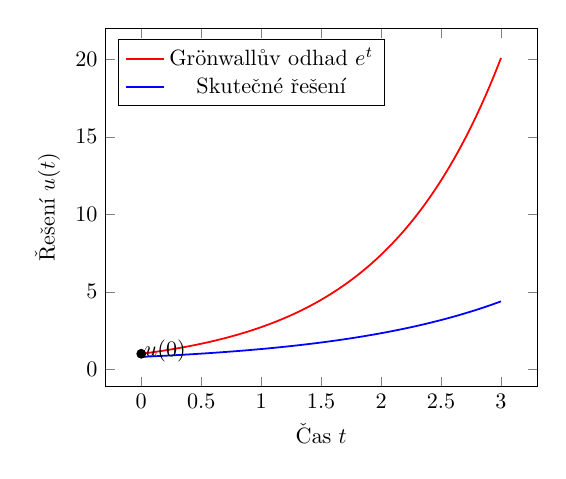
\begin{tikzpicture}[scale=0.8]
\begin{axis}[
    xlabel={Čas $t$},
    ylabel={Řešení $u(t)$},
    domain=0:3,
    samples=100,
    legend pos=north west
]
% Exponenciální horní odhad
\addplot[red, thick] {exp(x)};
\addlegendentry{Grönwallův odhad $e^t$}

% Skutečné řešení nerovnice
\addplot[blue, thick] {0.5*exp(0.7*x) + 0.3};
\addlegendentry{Skutečné řešení}

% Počáteční podmínka
\addplot[only marks, mark=*, mark size=2pt] coordinates {(0,1)};
\node at (axis cs:0.2,1.2) {$u(0)$};
\end{axis}
\end{tikzpicture}
\caption{Grönwallův odhad exponenciálního růstu řešení}
\label{fig:gronwall-estimate}
\end{figure}

\begin{example}[Aplikace na stabilitu řešení]
Uvažujme perturbovanou rovnici $y' = f(t,y) + g(t,y)$ s $\|g(t,y)\| \leq \epsilon$. Pokud $f$ je Lipschitzovská s konstantou $L$, pak rozdíl řešení $\Delta y$ splňuje:
\[
\|\Delta y(t)\| \leq \|\Delta y(0)\|e^{Lt} + \frac{\epsilon}{L}(e^{Lt} - 1)
\]
\end{example}

\begin{keyinsight}
Grönwallovo lemma je univerzální nástroj pro stabilitní analýzu - umožňuje převést lokální odhady na globální a kontrolovat kumulaci chyb v čase. Je fundamentální pro teorii robustness a citlivosti dynamických systémů.
\end{keyinsight}

\begin{summary}
\textbf{Klíčové koncepty:} Diferenciální a integrální forma, exponenciální odhady. \\
\textbf{Hlavní výsledky:} Různé varianty Grönwallova lemmatu. \\
\textbf{Aplikace:} Analýza stability, odhady perturbací, kontrola chyb.
\end{summary}

\spc

\subsection{Peanova existenční věta: Existence bez jednoznačnosti}

\begin{scaffold}
\textbf{Co umíme:} Picardova věta vyžaduje Lipschitzovskost pro jednoznačnost. \\
\textbf{Co se naučíme:} Existenci řešení za obecnějších podmínek. \\
\textbf{K čemu to využijeme:} Analýza systémů s více režimy chování.
\end{scaffold}

\begin{motivation}
Peanova věta umožňuje existenci řešení i tam, kde Lipschitzovskost neplatí - například pro systémy s nespojitostmi nebo rychle oscilujícími pravými stranami. Tato obecnost je důležitá pro aplikace v teorii řízení a hybridních systémech.
\end{motivation}

\begin{theorem}[Peanova existenční věta]
Nechť $f: [t_0, t_0+a] \times \overline{B(y_0,b)} \to \mathbb{R}^n$ je spojitá a omezená. Pak počáteční úloha
\[
y' = f(t,y), \quad y(t_0) = y_0
\]
má alespoň jedno řešení na intervalu $[t_0, t_0+h]$, kde $h = \min\left(a, \frac{b}{M}\right)$, $M = \sup\|f(t,y)\|$.
\end{theorem}

\begin{proof}[Náčrt důkazu]
\begin{enumerate}
\item Konstrukce Eulerovy lomené čáry:
\begin{align*}
t_k &= t_0 + \frac{kh}{n}, \quad k = 0,1,\dots,n \\
\phi_n(t) &= y_0 + \int_{t_0}^t f(s, \phi_n(s))\, ds \quad \text{na sítích}
\end{align*}
\item Rovnoměrná omezenost a stejnoměrná spojitost: $\|\phi_n(t)\| \leq b$, $\|\phi_n(t) - \phi_n(s)\| \leq M|t-s|$
\item Arzelà-Ascoliho věta: Existuje stejnoměrně konvergentní podposloupnost $\phi_{n_k} \to \phi$
\item Limita splňuje integrální rovnici, tedy i diferenciální rovnici
\end{enumerate}
\qed
\end{proof}

\begin{intuition}
Peanova konstrukce používá Eulerovu lomenou čáru - aproximujeme řešení po malých krocích. I když tyto aproximace nemusejí konvergovat k jediné limitě (kvůli chybějící jednoznačnosti), některá podposloupnost konverguje k řešení.
\end{intuition}

\begin{example}[Případ bez jednoznačnosti]
Uvažujme rovnici $y' = 2\sqrt{|y|}$, $y(0) = 0$. Tato rovnice má nekonečně mnoho řešení:
\[
y(t) = 0 \quad \text{a} \quad y(t) = \begin{cases}
0 & t \leq c \\
(t-c)^2 & t > c
\end{cases}
\]
pro libovolné $c \geq 0$. Funkce $\sqrt{|y|}$ není Lipschitzovská v nule.
\end{example}

\begin{keyinsight}
V kvantových systémech může volba parametru $c$ odpovídat různým časům přechodu mezi kvantovými stavy nebo různým měřicím protokolům. Existence více řešení odráží fundamentální nedeterminismus v některých kvantových procesech.
\end{keyinsight}

\begin{application}
V kvantové kontrole: Systémy s přepínáním mezi různými Hamiltoniány mohou mít více řešení odpovídajících různým řídicím strategiím. Peanova věta garantuje existenci alespoň jednoho řešení.
\end{application}

\begin{summary}
\textbf{Klíčové koncepty:} Eulerova lomená čára, Arzelà-Ascoliho věta. \\
\textbf{Hlavní výsledky:} Existence za podmínek spojitosti bez Lipschitzovskosti. \\
\textbf{Aplikace:} Systémy s nespojitostmi, hybridní dynamika, teorie řízení.
\end{summary}

\spc

\subsection{Carathéodoryho existenční věta: Zobecnění pro měřitelné pravé strany}

\begin{scaffold}
\textbf{Co umíme:} Peanova věta pro spojité pravé strany. \\
\textbf{Co se naučíme:} Teorii pro měřitelné, ne nutně spojité funkce. \\
\textbf{K čemu to využijeme:} Řízení, optimalizace, systémy s impulzy.
\end{scaffold}

\begin{motivation}
Mnohé aplikace v kvantové fyzice a ekonomii používají měřitelné integrandy - například systémy s okamžitými přepnutími, impulzní řízení, nebo modely s náhodnými vlivy. Carathéodoryho teorie rozšiřuje dosah ODR na tyto praktické scénáře.
\end{motivation}

\begin{theorem}[Carathéodoryho existenční věta]
Nechť $f: [t_0, t_0+a] \times \mathbb{R}^n \to \mathbb{R}^n$ splňuje:
\begin{enumerate}
\item Pro skoro všechna $t$ je $f(t,\cdot)$ spojitá
\item Pro každé $y$ je $f(\cdot,y)$ měřitelná
\item Existuje integrovatelná funkce $m(t)$ taková, že $\|f(t,y)\| \leq m(t)$ pro skoro všechna $t$ a všechna $y$
\end{enumerate}
Pak počáteční úloha $y' = f(t,y)$, $y(t_0) = y_0$ má řešení na $[t_0, t_0+a]$.
\qed
\end{theorem}

\begin{intuition}
Carathéodoryho podmínky umožňují pravé straně být "skoro všude" spojitá v čase a spojitá ve stavové proměnné. Absolutní spojitost řešení zaručuje, že derivace existuje skoro všude a řešení lze zrekonstruovat integrací.
\end{intuition}

\begin{example}[Aplikace v kvantové kontrole]
Uvažujme systém s přepínáním mezi Hamiltoniány:
\[
i\hbar\frac{d\psi}{dt} = \hat{H}_k(t)\psi, \quad t \in [t_k, t_{k+1}]
\]
kde přepínací časy $t_k$ tvoří měřitelnou množinu. Carathéodoryho věta garantuje existenci řešení.
\end{example}

\begin{keyinsight}
Carathéodoryho teorie rozšiřuje použití ODR na problémy s měřitelnými vstupy a řídicími strategiemi. To je klíčové pro moderní aplikace v teorii řízení, ekonomii a kvantové informaci.
\end{keyinsight}

\begin{summary}
\textbf{Klíčové koncepty:} Měřitelnost, absolutní spojitost, Carathéodoryho podmínky. \\
\textbf{Hlavní výsledky:} Existence pro měřitelné pravé strany. \\
\textbf{Aplikace:} Teorie řízení, ekonomické modely, hybridní systémy.
\end{summary}

\spc

\subsection{Prodloužování řešení a maximální interval existence}

\begin{scaffold}
\textbf{Co umíme:} Lokální existence řešení z předchozích vět. \\
\textbf{Co se naučíme:} Podmínky pro globální existenci a kritéria "blow-up". \\
\textbf{K čemu to využijeme:} Analýza dlouhodobého chování a detekce singularit.
\end{scaffold}

\begin{motivation}
V aplikacích potřebujeme vědět, zda lze řešení rozšířit na celý časový horizont, nebo zda v konečném čase "exploduje". Tato otázka je klíčová pro stabilitu modelů a bezpečnost řídicích systémů.
\end{motivation}

\begin{definition}[Maximální řešení a interval existence]
Řešení $\phi: I \to \mathbb{R}^n$ se nazývá \emph{maximální}, pokud neexistuje řešení $\psi: J \to \mathbb{R}^n$ s $I \subsetneq J$ a $\psi|_I = \phi$. Interval $I$ je \emph{maximální interval existence}.
\end{definition}

\begin{theorem}[Prodloužení řešení]
Nechť $f: D \subset \mathbb{R} \times \mathbb{R}^n \to \mathbb{R}^n$ je spojitá a $\phi: (\alpha, \beta) \to \mathbb{R}^n$ je maximální řešení. Pak buď $\beta = +\infty$, nebo pro každý kompakt $K \subset D$ existuje $t_K < \beta$ takové, že $(t, \phi(t)) \notin K$ pro $t > t_K$.
\qed
\end{theorem}

\begin{theorem}[Podmínky globální existence]
Je-li $f$ spojitá a existují funkce $\alpha, \beta: \mathbb{R} \to \mathbb{R}$ takové, že
\[
\|f(t,y)\| \leq \alpha(t)\|y\| + \beta(t)
\]
s $\alpha, \beta$ spojitými na $\mathbb{R}$, pak každé maximální řešení existuje na celém $\mathbb{R}$.
\qed
\end{theorem}

\begin{intuition}
Řešení lze prodlužovat, dokud zůstává v kompaktní oblasti. Pokud řešení "uteče do nekonečna" v konečném čase, nastává blow-up. Lineární růst pravé strany zaručuje, že řešení nemůže explodovat v konečném čase.
\end{intuition}

\begin{figure}[htbp]
\centering
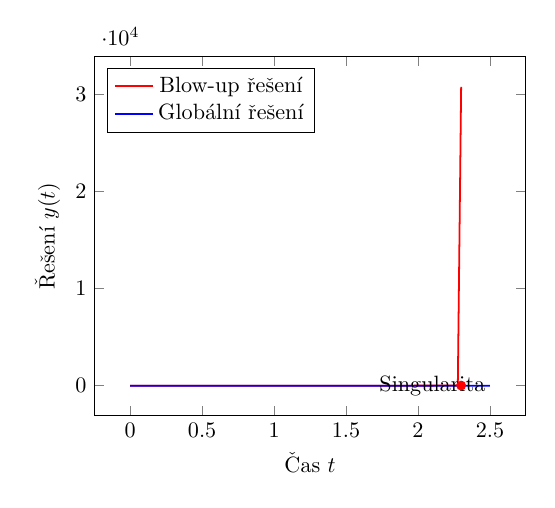
\begin{tikzpicture}[scale=0.8]
\begin{axis}[
    xlabel={Čas $t$},
    ylabel={Řešení $y(t)$},
    domain=0:2.5,
    samples=100,
    legend pos=north west
]
% Blow-up řešení
\addplot[red, thick, domain=0:2.3] {1/(2.3-x)};
\addlegendentry{Blow-up řešení}

% Globální řešení
\addplot[blue, thick] {1 + 0.3*x};
\addlegendentry{Globální řešení}

% Singularita
\addplot[only marks, mark=*, mark size=2pt, red] coordinates {(2.3,8)};
\node at (axis cs:2.1,9) {Singularita};
\end{axis}
\end{tikzpicture}
\caption{Porovnání blow-up a globálního řešení}
\label{fig:blowup-global}
\end{figure}

\begin{example}[Blow-up v nelineární Schrödingerově rovnici]
Pro NLS $i\psi_t + \psi_{xx} + |\psi|^2\psi = 0$ s dostatečně velkou počáteční podmínkou může dojít k blow-up v konečném čase: $\|\psi(t)\|_{L^\infty} \to \infty$ pro $t \to T^-$.
\end{example}

\begin{keyinsight}
Kontrola parametrů a počátečních podmínek může zaručit globální existenci řešení. Pro systémy s potenciálním blow-up je důležité stanovit kritéria, kdy k explozi dochází a kdy ne.
\end{keyinsight}

\begin{summary}
\textbf{Klíčové koncepty:} Maximální řešení, interval existence, blow-up. \\
\textbf{Hlavní výsledky:} Věty o prodlužování, podmínky globální existence. \\
\textbf{Aplikace:} Analýza stability, detekce singularit, kvantová teorie pole.
\end{summary}

\spc

\subsection{Spojitá a hladká závislost na datech a parametrech}

\begin{scaffold}
\textbf{Co umíme:} Existence a jednoznačnost řešení. \\
\textbf{Co se naučíme:} Citlivost řešení na změny vstupů a parametrů. \\
\textbf{K čemu to využijeme:} Bifurkační analýza, optimalizace, robustní řízení.
\end{scaffold}

\begin{motivation}
V kvantových experimentech i technických aplikacích jsou vstupní parametry a počáteční podmínky známy pouze přibližně. Potřebujeme vědět, jak malé chyby v těchto údajích ovlivní řešení.
\end{motivation}

\begin{theorem}[Spojitá závislost na počátečních podmínkách]
Nechť $f$ je spojitá a lokálně Lipschitzovská. Pak řešení $y(t; t_0, y_0)$ závisí spojitě na počáteční podmínce $y_0$. Konkrétně, pro kompaktní interval $I$ existuje $L$ takové, že
\[
\|y(t; t_0, y_0) - y(t; t_0, z_0)\| \leq \|y_0 - z_0\|e^{L|t-t_0|}
\]
\end{theorem}

\begin{theorem}[Hladká závislost na parametrech]
Nechť $f(t,y,\lambda)$ je $C^k$ v $(y,\lambda)$. Pak řešení $y(t;\lambda)$ je $C^k$ v $\lambda$.
\qed
\end{theorem}

\begin{intuition}
Spojitá závislost znamená, že malá změna vstupů vede k malé změně řešení. Hladká závislost umožňuje použít derivační metody pro analýzu citlivosti a optimalizaci.
\end{intuition}

\begin{example}[Derivace řešení podle parametru]
Pro rovnici $y' = f(t,y,\lambda)$, $y(0) = y_0$ platí variační rovnice:
\[
\frac{\partial}{\partial t}\left(\frac{\partial y}{\partial\lambda}\right) = D_y f(t,y,\lambda)\frac{\partial y}{\partial\lambda} + D_\lambda f(t,y,\lambda)
\]
s počáteční podmínkou $\frac{\partial y}{\partial\lambda}(0) = 0$.
\end{example}

\begin{keyinsight}
Diferenciovatelná závislost řešení na parametrech je klíčová pro optimalizační problémy a analýzu citlivosti. Umožňuje použít gradientní metody a studovat stabilitu řešení vůči perturbacím.
\end{keyinsight}

\begin{application}
V bifurkační analýze: Hladká závislost na parametrech umožňuje studovat, jak se kvalitativní chování systému mění s parametry. Body, kde derivace neexistuje, často odpovídají bifurkačním bodům.
\end{application}

\begin{summary}
\textbf{Klíčové koncepty:} Spojitá závislost, hladká závislost, derivace řešení. \\
\textbf{Hlavní výsledky:} Věty o spojité a hladké závislosti. \\
\textbf{Aplikace:} Bifurkační analýza, optimalizace, studie citlivosti.
\end{summary}

\spc

\subsection{Wazewskiho topologická metoda}

\begin{scaffold}
\textbf{Co umíme:} Analytické metody existence z předchozích vět. \\
\textbf{Co se naučíme:} Topologický přístup k existenci řešení. \\
\textbf{K čemu to využijeme:} Nehomogenní a okrajové úlohy, systémy s vícero řešeními.
\end{scaffold}

\begin{motivation}
Topologické metody doplňují čistě analytické důkazy existence a jsou zvláště účinné pro problémy s okrajovými podmínkami nebo systémy, kde analytické podmínky jsou obtížně ověřitelné.
\end{motivation}

\begin{definition}[Wazewskiho množina]
Množina $W \subset \mathbb{R} \times \mathbb{R}^n$ se nazývá \emph{Wazewskiho množina} pro rovnici $y' = f(t,y)$, jestliže:
\begin{itemize}
\item Je-li $(t_0, y_0) \in W$ a řešení opustí $W$ v čase $t_1 > t_0$, pak opustí přes hranici $\partial W$
\item Množina okamžitého úniku je uzavřená v $\partial W$
\end{itemize}
\end{definition}

\begin{theorem}[Wazewskiho princip]
Nechť $W$ je Wazewskiho množina a existuje podmnožina $Z \subset \partial W$ taková, že:
\begin{itemize}
\item Žádné řešení neopouští $W$ přes $Z$
\item $Z$ je deformačním retraktem $W$ ale není deformačním retraktem $W \cup Z$
\end{itemize}
Pak existuje řešení, které zůstává v $W$ pro všechna $t \geq t_0$.
\qed
\end{theorem}

\begin{intuition}
Wazewskiho princip je topologická verze "pastí na řešení" - pokud řešení nemůže uniknout určitými částmi hranice, musí existovat řešení, které zůstane uvnitř množiny.
\end{intuition}

\begin{application}
V kvantové mechanice: Wazewskiho metoda může garantovat existenci vázaných stavů v nehomogenních potenciálech nebo existenci periodických orbit v kvantových dotacích.
\end{application}

\begin{keyinsight}
Topologické metody rozšiřují dosah existenčních teorémů na problémy, kde analytické podmínky jsou obtížně ověřitelné. Poskytují kvalitativní kritéria existence bez nutnosti explicitní konstrukce řešení.
\end{keyinsight}

\begin{summary}
\textbf{Klíčové koncepty:} Wazewskiho množina, topologický princip, deformační retrakt. \\
\textbf{Hlavní výsledky:} Wazewskiho princip existence řešení. \\
\textbf{Aplikace:} Okrajové úlohy, periodická řešení, kvalitativní analýza.
\end{summary}

\spc

\subsection{Diferenciální inkluze a jejich aplikace}

\begin{scaffold}
\textbf{Co umíme:} Jednohodnotový přístup k ODR. \\
\textbf{Co se naučíme:} Multi-valued dynamiku a její vlastnosti. \\
\textbf{K čemu to využijeme:} Teorie řízení, stochastické modely, hybridní systémy.
\end{scaffold}

\begin{motivation}
Mnohé reálné systémy - jako systémy s přepínáním, s hysterézí, nebo s neurčitými parametry - nelze adekvátně modelovat jednohodnotovými ODR. Diferenciální inkluce poskytují framework pro takové multi-valued dynamiky.
\end{motivation}

\begin{definition}[Diferenciální inkluze]
\emph{Diferenciální inklucí} rozumíme problém
\[
y'(t) \in F(t, y(t)), \quad y(t_0) = y_0
\]
kde $F: \mathbb{R} \times \mathbb{R}^n \to 2^{\mathbb{R}^n}$ je multi-valued zobrazení.
\end{definition}

\begin{theorem}[Filippovova existenční věta]
Nechť $F$ je multi-valued zobrazení splňující:
\begin{itemize}
\item $F(t,y)$ je neprázdná, konvexní a kompaktní pro všechna $(t,y)$
\item $F$ je měřitelné v $t$ a Lipschitzovské v $y$
\item $\|F(t,y)\| \leq m(t)(1 + \|y\|)$ pro integrovatelnou $m(t)$
\end{itemize}
Pak diferenciální inkluce má řešení na $[t_0, t_0+a]$.
\qed
\end{theorem}

\begin{intuition}
Diferenciální inkluce modelují systémy, kde v každém okamžiku může být rychlost změny stavu vybrána z určité množiny možností. To odpovídá situacím s nedeterministickým chováním nebo více možnými režimy.
\end{intuition}

\begin{example}[Filippovova regularizace]
Pro systém s přepínáním $y' = f_1(y)$ pro $h(y) > 0$, $y' = f_2(y)$ pro $h(y) < 0$ definujeme Filippovovu inkluci na přepínací hranici $h(y) = 0$:
\[
y' \in \overline{\text{co}}\{f_1(y), f_2(y)\}
\]
\end{example}

\begin{keyinsight}
Konvexní uzávěr v Filippovově regularizaci zajišťuje existenci řešení na přepínacích hranicích a zachovává fyzikální interpretaci hybridních kvantových systémů, kde přechody mezi stavy mohou být spojité.
\end{keyinsight}

\begin{application}
V hybridní kvantové kontrole: Systémy přepínající mezi různými Hamiltoniány podle měření lze modelovat diferenciálními inklucemi, kde množina $F(t,\psi)$ obsahuje všechny možné Hamiltoniány kompatibilní s aktuálním měřením.
\end{application}

\begin{summary}
\textbf{Klíčové koncepty:} Multi-valued zobrazení, diferenciální inkluze, Filippovova regularizace. \\
\textbf{Hlavní výsledky:} Existenční věty pro diferenciální inkluze. \\
\textbf{Aplikace:} Hybridní systémy, teorie řízení, systémy s přepínáním.
\end{summary}

\spc

\subsection*{Shrnutí kapitoly}

\begin{itemize}
\item Představili jsme fundamentální teorémy existence a jednoznačnosti řešení ODR
\item Picardova-Lindelöfova věta poskytuje konstruktivní důkaz za Lipschitzovských podmínek
\item Peanova a Carathéodoryho věta rozšiřují existenci na obecnější třídy pravých stran
\item Grönwallovo lemma je univerzální nástroj pro odhady a analýzu stability
\item Teorie prodlužování řešení popisuje podmínky globální existence a kritéria blow-up
\item Spojitá a hladká závislost na parametrech je klíčová pro analýzu citlivosti
\item Topologické metody a diferenciální inkluce rozšiřují dosah klasické teorie
\end{itemize}

\vspace{0.5cm}

\begin{tcolorbox}[title=\textbf{Doporučená literatura}, colback=blue!5!white, colframe=blue!75!black]
\begin{itemize}
\item \textbf{Hartman, P.} \emph{Ordinary Differential Equations}
\item \textbf{Hale, J. K.} \emph{Ordinary Differential Equations}  
\item \textbf{Coddington, E. A.; Levinson, N.} \emph{Theory of Ordinary Differential Equations}
\item \textbf{Filippov, A. F.} \emph{Differential Equations with Discontinuous Righthand Sides}
\end{itemize}
\end{tcolorbox}

\begin{transition}
V \hyperref[sec:pokrocila-teorie]{Kapitole 4} prohloubíme kvalitativní analýzu dynamických systémů pomocí teorie stability, bifurkací a Ljapunovových metod. Aplikujeme získané výsledky na studium dlouhodobého chování řešení a přechodů mezi různými režimy dynamiky.
\end{transition}

\spc